\chapter{Experiments and results}
\label{chap:experiments_and_results}
\besk{Et kapittel der du har satt opp (med hyper-parametere og miljø-variabler f.eks. i en oversiktlig tabell) eksperimenter, kjørt simulation-runs med disse verdiene, og viser hva resultatene ble. Resultater kan være \textbf{performance-plot}s (ift. harmonic synch.-times for diverse hyper-parametere og miljøvariabler (samt om robotene er homogene eller heterogene og isåfall hvordan), der plottet må lages spesifikt for hvert eksperiment, og kan f.eks. være boxplot eller tabeller med performance-/hsynchtime-/simulation-time(s)-verdier), \textbf{performance-measure plot}s (altså hvordan harmonic synch. ble detectet i et simulation-run, med \textit{plot\_PerformanceMeasurePlot\_for\_SimRun.py}), \textbf{phase-\&frequency-plot}s (altså hvilke fase- og frekvens-verdier robotene hadde iløpet av simulation-run'et, via \textit{plot\_PhaseFrequencyPlot\_for\_SimRun.py}), eller \textbf{synchrony-evolution plot}s (der 'towards\_k\_counter'en iløpet av simulation-run'et plottes, via \textit{plot\_SynchronyEvolutionPlot\_for\_SimRun.py})}

\besk{Helst gode eksperimenter som motiveres og forklares, settes opp, og utføres m/resultater man diskuterer og analyserer. Det er bra å evaluere fra flere synspunkt \tcol[gray]{med flere research methods og hvis tid}}

	\section{Solving the simpler $\phi-$problem}
	This is the section for the experiments attempting to solve the first and simpler problem, namely synchronizing the phases $\phi_i$ of all agents $i$. \nl
	
	\subsection{Reproducing K. Nymoen's phase synchronization}
	In order to see that our developed synchronization simulator in Unity yields more or less the same results as K. Nymoen et al.'s firefly system \cite{nymoen_synch}, similar experiments as reported in their paper are performed. These tell us whether differences in performance, in terms of synchronization times (s), is simply due to implementation differences, or actually because of the synchronization methods and hyperparameters in question. First off, for the $\phi$ problem of synchronizing only phases (i.e. already having synchronized frequencies), K. Nymoen et al.'s phase adjustment method (presented in Section \ref{nymoen_phase_adjust}) will be experimented with for varying phase coupling constants $\alpha$, as also performed and reported in their paper (c.f. their Fig. 7). \nl
	
	\tcol[blue]{FYLL INN}
	
	\begin{figure}[ht!]
		\centering
		% \includegraphics[width=0.7\]{Assets/DocSegments/Chapters/ExperimentsAndResults/Figures/}
		\caption{Synchronization times (s) for 6 robots with initially random and unsynchronized phases but equal and fixed frequencies (1Hz), with varying $\alpha$ values. 30 simulation runs per $\alpha$ value.}
	\end{figure}
	
	
	\subsection{Hyperparameter search}
	
	\subsection{Comparing phase adjustment methods}
	Now, an experiment follows where we investigate the validity of the claimed [] benefits of performing bi directional phase adjustments—both inhibitory and excitatory—compared to simply adjusting phases in an excitatory way (i.e. only ``pushing'' other ocillators's phase higher when firing, not ``holding back'').
	
	% \begin{figure}[ht!]
		% \centering
		% 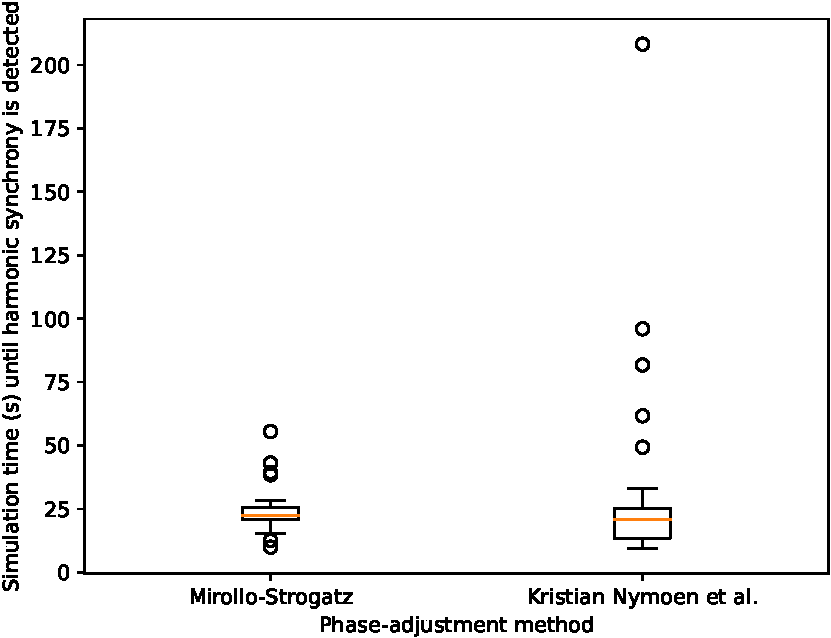
\includegraphics[width=0.7\linewidth]{Assets/DocSegments/Chapters/ExperimentsAndResults/Figures/FirstAndFaultyExperimentPlot.pdf}
		% \caption[Performance-plot from initial simulator-experiment]{Performance-plot: harmonic synchronization-times from initial simulator-experiment when synchronizing phases $\phi_i$ for all agents $i$, where all phases are initially uniformly randomized between 0 and 1, and eventually synchronize and align. We here measure how long it takes 6 agents to synchronize their phases to each other, given the two different phase-adjustment methods. 30 individual runs per phase-adjustment method were performed in Unity for a collective-size of 6 agents, and $\alpha=0.2$ e.g.}
		% \label{fig:EPA1}
	% \end{figure}
	
	
	
	
	
	\section{Solving the harder $\phi\&\omega-$problem}
	
	This is the section for the experiments attempting to solve the second and harder problem of synchronizing both phases $\phi_i$, as well as frequencies $\omega_i$, for all agents $i$.
	
	\subsection{Reproducing K. Nymoen's frequency synchronization}
	
	\subsection{Hyperparameter search?}